%%%%%%%%%%%%%%%%%%%%%%%%%%%%%%%%%%%%%%%%%
% Beamer Presentation
% LaTeX Template
% Version 1.0 (10/11/12)
%
% This template has been downloaded from:
% http://www.LaTeXTemplates.com
%
% License:
% CC BY-NC-SA 3.0 (http://creativecommons.org/licenses/by-nc-sa/3.0/)
%
%%%%%%%%%%%%%%%%%%%%%%%%%%%%%%%%%%%%%%%%%

%----------------------------------------------------------------------------------------
%	PACKAGES AND THEMES
%----------------------------------------------------------------------------------------

\documentclass[9pt, t]{beamer}

%% Packages
\usepackage{multicol}
\usepackage[english]{babel}
\usepackage{eurosym}
\usepackage{etex}
\usepackage{pgfpages}
\usepackage[utf8]{inputenc}
\usepackage[T1]{fontenc}
\usepackage{hyperref}
\usepackage{alltt}
\usepackage{color}
\usepackage{amsmath,amsfonts,amssymb,amsthm}
\usepackage[ruled,vlined]{algorithm2e}
\usepackage{xspace}
\usepackage[normalem]{ulem}
\usepackage{filemod}
%\usepackage{bibentry}
\usepackage{multicol}
\usepackage[absolute,overlay]{textpos}
\usepackage{array}
\newcounter{chapter} 
\usepackage[framemethod=TikZ]{mdframed}
\usepackage[backend=biber]{biblatex}
\addbibresource{bib.bib}


\usepackage{listings}
\lstset{
  basicstyle=\ttfamily,
  columns=fullflexible,
  keywordstyle=\color{red}\bfseries,
  commentstyle=\color{purple},
  keepspaces=true,
  showstringspaces=false,
  tabsize=4,
  escapeinside={<@}{@>},
}

\mode<presentation> {
  \usetheme[secheader]{Boadilla}
  \usecolortheme{beaver}
  \usefonttheme{serif}

  \colorlet{custom}{beamerstructure}

  \definecolor{DarkBlue}{RGB}{20,20,255}
  \definecolor{DarkRed}{RGB}{220,10,10}
  \definecolor{Ocra}{RGB}{255,255,204}
  \definecolor{VeryLightGray}{RGB}{242,242,242}

  \setbeamertemplate{navigation symbols}{}
  \setbeamercolor{alerted text}{fg=DarkRed,bg=Ocra}

  \setbeamercolor{itemize subitem}{fg=blue}
  \setbeamertemplate{itemize subitem}[ball]
  \setbeamercolor{itemize subsubitem}{fg=blue}
  \setbeamertemplate{itemize subsubitem}[ball]

  \setbeamercolor*{palette primary}{use=structure,fg=black,bg=structure.fg!20}
  \setbeamercolor*{palette secondary}{use=structure,fg=black,bg=structure.fg!40}
  \setbeamercolor*{palette tertiary}{use=structure,fg=white,bg=structure.fg!70}
  \setbeamercolor*{palette quaternary}{fg=white,bg=black}

  \setbeamercolor{block body}{bg=gray!20}
  \setbeamercolor{frametitle}{bg=gray!20}
  \setbeamercolor{block title}{bg=blue!20,fg=black}
}

\usepackage{graphicx} % Allows including images
\usepackage{booktabs} % Allows the use of \toprule, \midrule and \bottomrule in tables

\graphicspath{{assets/}}

%----------------------------------------------------------------------------------------
%	TITLE PAGE
%----------------------------------------------------------------------------------------

\title[Signal Image \& Video]{Skeletonization of Binary Images} % The short title appears at the bottom of every slide, the full title is only on the title page

\author{Filippo Momesso} % Your name
\institute[UniTN] % Your institution as it will appear on the bottom of every slide, may be shorthand to save space
{
University of Trento \\ % Your institution for the title page
\medskip
\textit{filippo.momesso@studenti.unitn.it} % Your email address
}
\date{\today} % Date, can be changed to a custom date

\begin{document}

\begin{frame}
  \titlepage % Print the title page as the first slide
\end{frame}

\begin{frame}
  \frametitle{Overview} % Table of contents slide, comment this block out to remove it
  \tableofcontents % Throughout your presentation, if you choose to use \section{} and \subsection{} commands, these will automatically be printed on this slide as an overview of your presentation
\end{frame}

%----------------------------------------------------------------------------------------
%	PRESENTATION SLIDES
%----------------------------------------------------------------------------------------

%-----------------------------------------------
\section{Basic definitions}
\begin{frame}
  \frametitle{What is Skeletonization?}
  \begin{block}{Skeletonization}
    An image processing technique which reduces a binary object (or region) to a 1 pixel wide representation called \textbf{skeleton}.
  \end{block}
  Useful in many application fields such as \emph{shape recognition and analysis}, \emph{animation}, \emph{motion tracking} or \emph{medical imaging}~\cite{skel-applications}.
  \begin{figure}
    \begin{center}
      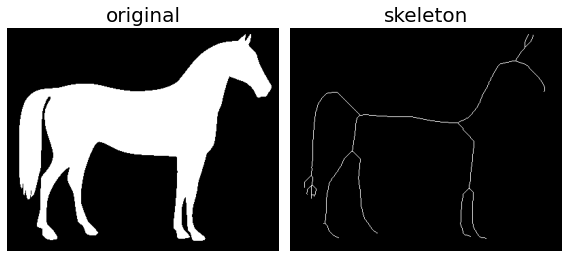
\includegraphics[width=0.6\textwidth]{skeletonization-example.png}
      \caption{Example of a skeletonized image.}
    \end{center}
  \end{figure}
\end{frame}

\begin{frame}
  \frametitle{Skeleton}
  \begin{block}{Skeleton}
    The ideal skeleton should:
    \begin{itemize}
      \item be a connected subset of points from the original region,
      \item represent the geometric characteristics of the region,
      \item preserve the topological characteristics of the region (e.g. connectivity, holes, cavities...)
    \end{itemize}
  \end{block}

  Three major skeletonization techniques:
  \begin{itemize}
    \item Medial-axis distance transform
    \item Non-pixel-based methods (computes analytically the skeleton)
    \item Thinning methods.
  \end{itemize}
  \vspace{0.5cm}
  We will focus on \textbf{thinning methods} since they are quite efficient and commonly used in state-of-the-art applications.
\end{frame}

\section{Zhang-Guo Parallalel Thinning}
\begin{frame}
  \frametitle{Input}
  \begin{block}

  \end{block}
\end{frame}

\section{Morphological Thinning}

\section{Lee's 3D Skeletonization}

\section{Wrap-up}
\begin{frame}
  \frametitle{Bibliography}
  \printbibliography
\end{frame}
\begin{frame}
  \frametitle{Conclusion}
  \begin{center}
    \Huge Thank you for your attention.
  \end{center}
\end{frame}
\end{document}
